
\begin{frame}{Միջակայքային ներկելիության անհրաժեշտ պայմաններ}

\begin{theorem}[Հասրաթյան, Քամալյան, 1987]
Եթե $G$ մուլտիգրաֆը ունի միջակայքային ներկում, ապա $\chi^{\prime}(G)=\Delta(G)$:
\end{theorem}

\pause

\begin{theorem}[Հասրաթյան, Քամալյան, 1987]
Եթե $G$-ն համասեռ մուլտիգրաֆ է, ապա
\begin{description}
\item[(1)] $G\in \mathfrak{N}$ այն և միայն այն դեպքում, երբ $\chi^{\prime}(G)=\Delta(G)$:
\item[(2)] Եթե $G\in \mathfrak{N}$ և $w(G)\leq t\leq W(G)$, ապա $G$-ն ունի միջակայքային $t$-ներկում:
\end{description}
\end{theorem}

\end{frame}

\begin{frame}{Միջակայքային ներկելիության անհրաժեշտ պայմաններ}

Աշխատանքում ստացվել է միջակայքային ներկելիության մեկ այլ անհրաժեշտ պայման:
\begin{theorem}[1.1.3]
Եթե $G$ մուլտիգրաֆի համար գոյություն ունի $d$ թիվ, որը $G$-ի բոլոր գագաթների աստիճանների ընդհանուր բաժանարար է, սակայն $\vert E(G)\vert$-ի բաժանարար չէ, ապա $G\notin \mathfrak{N}$:
\end{theorem}
\pause
\begin{corollary}[1.1.4]
Եթե $G$-ն էյլերյան մուլտիգրաֆ է և $\vert
E(G)\vert$ կենտ է, ապա $G\notin \mathfrak{N}$:
\end{corollary}
\end{frame}

\begin{frame}{Միջակայքային ներկելիության անհրաժեշտ պայմաններ}{Օրինակներ}

\begin{figure}[h]
\centering
\begin{subfigure}{.5\textwidth}
  \centering
  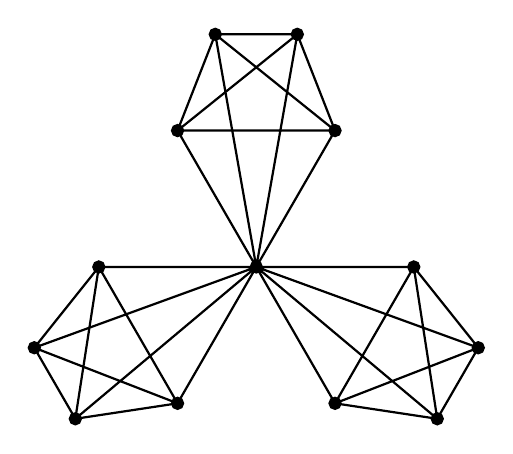
\begin{tikzpicture}[style=thick]
    \coordinate (V0) at (0:0cm);
    \coordinate (V1_1) at (120:2cm);
    \coordinate (V1_2) at (100:3cm);
    \coordinate (V1_3) at (80:3cm);
    \coordinate (V1_4) at (60:2cm);
    \coordinate (V2_1) at (0:2cm);
    \coordinate (V2_2) at (-20:3cm);
    \coordinate (V2_3) at (-40:3cm);
    \coordinate (V2_4) at (-60:2cm);
    \coordinate (V3_1) at (-120:2cm);
    \coordinate (V3_2) at (-140:3cm);
    \coordinate (V3_3) at (-160:3cm);
    \coordinate (V3_4) at (-180:2cm);
    
    \draw (V0) -- (V1_1) -- (V1_3) -- (V0) -- (V1_2) -- (V1_4) -- (V1_1) -- (V1_2) -- (V1_3) -- (V1_4) -- (V0)
    -- (V2_1) -- (V2_3) -- (V0) -- (V2_2) -- (V2_4) -- (V2_1) -- (V2_2) -- (V2_3) -- (V2_4) -- (V0)
    -- (V3_1) -- (V3_3) -- (V0) -- (V3_2) -- (V3_4) -- (V3_1) -- (V3_2) -- (V3_3) -- (V3_4) -- (V0);
    
    \draw[fill=black] (V0) circle (2pt);
    \draw[fill=black] (V1_1) circle (2pt);
    \draw[fill=black] (V1_2) circle (2pt);
    \draw[fill=black] (V1_3) circle (2pt);
    \draw[fill=black] (V1_4) circle (2pt);
    \draw[fill=black] (V2_1) circle (2pt);
    \draw[fill=black] (V2_2) circle (2pt);
    \draw[fill=black] (V2_3) circle (2pt);
    \draw[fill=black] (V2_4) circle (2pt);
    \draw[fill=black] (V3_1) circle (2pt);
    \draw[fill=black] (V3_2) circle (2pt);
    \draw[fill=black] (V3_3) circle (2pt);
    \draw[fill=black] (V3_4) circle (2pt);
 \end{tikzpicture}
\end{subfigure}%
\begin{subfigure}{.5\textwidth}
  \centering
  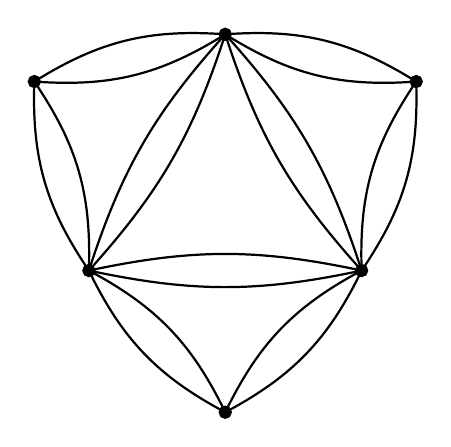
\begin{tikzpicture}[style=thick]
    \coordinate (V1) at (90:2cm);
    \coordinate (V2) at (-150:2cm);
    \coordinate (V3) at (-30:2cm);
    \coordinate (V12) at (150:2.8cm);
    \coordinate (V13) at (30:2.8cm);
    \coordinate (V23) at (-90:2.8cm);
    
    \draw (V1) edge[bend left=18] (V13);
    \draw (V1) edge[bend left=-18] (V13);
    \draw (V1) edge[bend left=18] (V12);
    \draw (V1) edge[bend left=-18] (V12);
    \draw (V1) edge[bend left=12] (V3);
    \draw (V1) edge[bend left=-12] (V3);
    \draw (V1) edge[bend left=12] (V2);
    \draw (V1) edge[bend left=-12] (V2);
    
    \draw (V2) edge[bend left=18] (V23);
    \draw (V2) edge[bend left=-18] (V23);
    \draw (V2) edge[bend left=18] (V12);
    \draw (V2) edge[bend left=-18] (V12);
    \draw (V2) edge[bend left=12] (V3);
    \draw (V2) edge[bend left=-12] (V3);
    
    \draw (V3) edge[bend left=18] (V23);
    \draw (V3) edge[bend left=-18] (V23);
    \draw (V3) edge[bend left=18] (V13);
    \draw (V3) edge[bend left=-18] (V13);
    
    \draw[fill=black] (V1) circle (2pt);
    \draw[fill=black] (V2) circle (2pt);
    \draw[fill=black] (V3) circle (2pt);
    \draw[fill=black] (V12) circle (2pt);
    \draw[fill=black] (V13) circle (2pt);
    \draw[fill=black] (V23) circle (2pt);
 \end{tikzpicture}
  
\end{subfigure}
\end{figure}
\end{frame}
